% Options for packages loaded elsewhere
\PassOptionsToPackage{unicode}{hyperref}
\PassOptionsToPackage{hyphens}{url}
\PassOptionsToPackage{dvipsnames,svgnames*,x11names*}{xcolor}
%
\documentclass[
  10pt,
  dvipsnames,enabledeprecatedfontcommands]{scrartcl}
\usepackage{amsmath,amssymb}
\usepackage{lmodern}
\usepackage{ifxetex,ifluatex}
\ifnum 0\ifxetex 1\fi\ifluatex 1\fi=0 % if pdftex
  \usepackage[T1]{fontenc}
  \usepackage[utf8]{inputenc}
  \usepackage{textcomp} % provide euro and other symbols
\else % if luatex or xetex
  \usepackage{unicode-math}
  \defaultfontfeatures{Scale=MatchLowercase}
  \defaultfontfeatures[\rmfamily]{Ligatures=TeX,Scale=1}
\fi
% Use upquote if available, for straight quotes in verbatim environments
\IfFileExists{upquote.sty}{\usepackage{upquote}}{}
\IfFileExists{microtype.sty}{% use microtype if available
  \usepackage[]{microtype}
  \UseMicrotypeSet[protrusion]{basicmath} % disable protrusion for tt fonts
}{}
\usepackage{xcolor}
\IfFileExists{xurl.sty}{\usepackage{xurl}}{} % add URL line breaks if available
\IfFileExists{bookmark.sty}{\usepackage{bookmark}}{\usepackage{hyperref}}
\hypersetup{
  pdftitle={``Weight of Evidence, Evidential Completeness and Accuracy''},
  pdfauthor={Rafal Urbaniak and Marcello Di Bello},
  colorlinks=true,
  linkcolor=Maroon,
  filecolor=Maroon,
  citecolor=Blue,
  urlcolor=blue,
  pdfcreator={LaTeX via pandoc}}
\urlstyle{same} % disable monospaced font for URLs
\usepackage{graphicx}
\makeatletter
\def\maxwidth{\ifdim\Gin@nat@width>\linewidth\linewidth\else\Gin@nat@width\fi}
\def\maxheight{\ifdim\Gin@nat@height>\textheight\textheight\else\Gin@nat@height\fi}
\makeatother
% Scale images if necessary, so that they will not overflow the page
% margins by default, and it is still possible to overwrite the defaults
% using explicit options in \includegraphics[width, height, ...]{}
\setkeys{Gin}{width=\maxwidth,height=\maxheight,keepaspectratio}
% Set default figure placement to htbp
\makeatletter
\def\fps@figure{htbp}
\makeatother
\setlength{\emergencystretch}{3em} % prevent overfull lines
\providecommand{\tightlist}{%
  \setlength{\itemsep}{0pt}\setlength{\parskip}{0pt}}
\setcounter{secnumdepth}{5}
%\documentclass{article}

% %packages
 \usepackage{booktabs}
\usepackage{subcaption}
\usepackage{multirow}
\usepackage{colortbl}
\usepackage{graphicx}
\usepackage{longtable}
\usepackage{ragged2e}
\usepackage{etex}
%\usepackage{yfonts}
\usepackage{marvosym}
\usepackage[notextcomp]{kpfonts}
\usepackage{nicefrac}
\newcommand*{\QED}{\hfill \footnotesize {\sc Q.e.d.}}
\usepackage{floatrow}
%\usepackage[titletoc]{appendix}
%\renewcommand\thesubsection{\Alph{subsection}}

\usepackage[textsize=footnotesize]{todonotes}
\newcommand{\ali}[1]{\todo[color=gray!40]{#1}}
\newcommand{\mar}[1]{\todo[color=blue!40]{#1}}
\newcommand{\raf}[1]{\todo[color=olive!40]{#1}}
%\linespread{1.5}
\newcommand{\indep}{\!\perp \!\!\! \perp\!}


\setlength{\parindent}{10pt}
\setlength{\parskip}{1pt}


%language
\usepackage{times}
\usepackage{t1enc}
%\usepackage[utf8x]{inputenc}
%\usepackage[polish]{babel}
%\usepackage{polski}




%AMS
\usepackage{amsfonts}
\usepackage{amssymb}
\usepackage{amsthm}
\usepackage{amsmath}
\usepackage{mathtools}

\usepackage{geometry}
 \geometry{a4paper,left=35mm,top=20mm,}


%environments
\newtheorem{fact}{Fact}



%abbreviations
\newcommand{\ra}{\rangle}
\newcommand{\la}{\langle}
\newcommand{\n}{\neg}
\newcommand{\et}{\wedge}
\newcommand{\jt}{\rightarrow}
\newcommand{\ko}[1]{\forall  #1\,}
\newcommand{\ro}{\leftrightarrow}
\newcommand{\exi}[1]{\exists\, {_{#1}}}
\newcommand{\pr}[1]{\mathsf{P}(#1)}
\newcommand{\cost}{\mathsf{cost}}
\newcommand{\benefit}{\mathsf{benefit}}
\newcommand{\ut}{\mathsf{ut}}

\newcommand{\odds}{\mathsf{Odds}}
\newcommand{\ind}{\mathsf{Ind}}
\newcommand{\nf}[2]{\nicefrac{#1\,}{#2}}
\newcommand{\R}[1]{\texttt{#1}}
\newcommand{\prr}[1]{\mbox{$\mathtt{P}_{prior}(#1)$}}
\newcommand{\prp}[1]{\mbox{$\mathtt{P}_{posterior}(#1)$}}



\newtheorem{q}{\color{blue}Question}
\newtheorem{lemma}{Lemma}
\newtheorem{theorem}{Theorem}



%technical intermezzo
%---------------------

\newcommand{\intermezzoa}{
	\begin{minipage}[c]{13cm}
	\begin{center}\rule{10cm}{0.4pt}



	\tiny{\sc Optional Content Starts}
	
	\vspace{-1mm}
	
	\rule{10cm}{0.4pt}\end{center}
	\end{minipage}\nopagebreak 
	}


\newcommand{\intermezzob}{\nopagebreak 
	\begin{minipage}[c]{13cm}
	\begin{center}\rule{10cm}{0.4pt}

	\tiny{\sc Optional Content Ends}
	
	\vspace{-1mm}
	
	\rule{10cm}{0.4pt}\end{center}
	\end{minipage}
	}
%--------------------






















\newtheorem*{reply*}{Reply}
\usepackage{enumitem}
\newcommand{\question}[1]{\begin{enumerate}[resume,leftmargin=0cm,labelsep=0cm,align=left]
\item #1
\end{enumerate}}

\usepackage{float}

% \setbeamertemplate{blocks}[rounded][shadow=true]
% \setbeamertemplate{itemize items}[ball]
% \AtBeginPart{}
% \AtBeginSection{}
% \AtBeginSubsection{}
% \AtBeginSubsubsection{}
% \setlength{\emergencystretch}{0em}
% \setlength{\parskip}{0pt}






\usepackage[authoryear]{natbib}

%\bibliographystyle{apalike}



\usepackage{tikz}
\usetikzlibrary{positioning,shapes,arrows}

\ifluatex
  \usepackage{selnolig}  % disable illegal ligatures
\fi

\title{``Weight of Evidence, Evidential Completeness and Accuracy''}
\author{Rafal Urbaniak and Marcello Di Bello}
\date{}

\begin{document}
\maketitle

\hypertarget{motivations}{%
\section{Motivations}\label{motivations}}

\hypertarget{balance-vs.-weight}{%
\subsection{Balance vs.~weight}\label{balance-vs.-weight}}

Suppose we want to represent our uncertainty about a proposition in
terms of a single probability that we assign to it. It is not too
difficult to inspire the intuition that this representation does not
capture an important dimension of how our uncertainty connects with the
evidence we have or have not obtained. In a 1872 manuscript of
\emph{The Fixation of Belief} (W3 295) C. S. Peirce gives an example
meant to do exactly that.

\begin{quote} When we have drawn a thousand times, if about half have been white, we have great confidence in this result. We now feel pretty sure that, if we were to make a large number of bets upon the color of single beans drawn from the bag, we could approximately insure ourselves in the long run by betting each time upon the white, a confidence which would be entirely wanting if, instead of sampling the bag by 1000 drawings, we had done so by only two.
\end{quote}

\noindent The objection is not too complicated. Your best estimate of
the probability of \(W=\)`the next bean will be white' is .5 if half of
the beans you have drawn randomly so far have been white, no matter
whether you have drawn a thousand or only two of them. But this means
that expressing your uncertainty about \(W\) by locutions such as "my
confidence in \(W\) is .5' does not capture this intuitively important
distinction.

Similar remarks can be found in Peirce's 1878
\emph{Probability of Induction}. There, he also proposes to represent
uncertainty by at least two numbers, the first depending on the inferred
probability, and the second measuring the amount of knowledge obtained;
as the latter, Peirce proposed to use some dispersion-related measure of
error (but then suggested that an error of that estimate should also be
estimated and so, so that ideally more numbers representing errors would
be needed).

Peirce himself did not call this the weight of evidence (and in fact,
used the phrase rather to refer to the balance of evidence, W3 294)
{[}CITE KASSER 2015{]}. However, his criticism of such an oversimplified
representation of uncertainty anticipated what came to be called weight
of evidence by Keynes in his 1921 \emph{A Treatise on Probability}:

\begin{quote}
As the relevant evidence at our disposal increases, the magnitude of the
probability of the argument may either increase or decrease, according as the new knowledge strengthens the unfavourable or the favourable evidence; but something seems to have increased in either case,—we have a more substantial basis upon which to rest our conclusion. I express this by saying that an accession of new evidence increases the weight of an argument. New evidence will sometimes decrease the probability of an argument but it will always increase its `weight.' (p. 71)
\end{quote}

\noindent The key point is the same {[}CITE LEVI 2001{]}: the balance of
probability alone cannot characterize all important aspects of
evidential appraisal. Keynes also considered measuring weight of
evidence in terms of the variance of the posterior distribution of a
certain parameter, but was quite attached to the idea that weight should
increase with new information, even if the dispersion increase with new
evidence {[}TP 80-82{]}, and so he proposed only a very rough sketch of
a positive sketch. Moreover, as he was uncertain how a measure of weight
should be incorporated in further decision-making, the was skeptical
about the practical significance of the notion. {[}TP 83{]}

But what is this positive sketch? On one hand, Keynes {[}TP 58-59{]}
connects the notion of weight with relevance. Call evidence \(E\)
relevant to \(X\) given \(K\) just in case
\(\mathsf{Pr}(X\vert K \wedge E) \neq \mathsf{Pr}(X \vert K)\).\footnote{
  Keynes also uses a slightly more convoluted notion of relevance to
  avoid equally strong items of opposite evidence turning out to be
  irrelevant (this objection has also been brought up by {[}COHEN 1986
  TWELVE{]}). The more complex version is that a proposition \(E_1\) is
  relevant to \(X\) given \(K\) just in case it entails a proposition
  \(E_2\) such that
  \(\pr{X\vert K \wedge E_2} \neq \mathsf{Pr}(X \vert K)\). {[}COHEN
  1986 TWELVE{]} complaints that this still runs into difficulties.
  Ignore \(K\), take an irrelevant proposition \(Z\). It entails
  \(Z\vee X\) and \(\pr{Z \vee X\vert X \wedge E}=1\). Now, by Bayes'
  theorem we have
  \(\pr{X \vert E \wedge (Z \vee X)} = \frac{\pr{X \vert E}\times \pr{Z \vee X \vert X \wedge E}}{\pr{Z \vee X \vert E}} = \frac{\pr{X \vert E}}{\pr{Z \vee X \vert E}}\).
  If the denominator differs from 1, the result differs from the
  numerator. We will ignore such difficulties, as they are not of key
  importance for the development of this chapter.} One postulate than
can be found in the \emph{Treatise} {[}TP 84{]} is:\footnote{RUNDE 1990
  283 suggests Keynes allows for weight of evidence to decrease when new
  evidence increases the range of alternatives, but this is based on
  Keynes' claim that weight is increased when the number of alternatives
  is reduced, and Keynes does not directly say anything about the
  possibility of an increase of the number of alternatives.}

\begin{tabular}{lp{11cm}}
(Monotonicity) & If $E$ is relevant to $X$ given $K$, where $K$ is background knowledge, $V(X\vert K \wedge E) > V(X\vert K)$, where $V$ is the weight of evidence.
\end{tabular}

{[}RUNDE 1990, 280{]} suggests that Keynes at some point calls weight
the completeness of information. This however, is a bit hasty, as Keynes
only says that
\emph{the degree of completeness of the information on which a probability is based does seem to be relevant, as well as the actual magnitude of the probabiltiy, in making practical decisions}.
As later on we will argue that it is actually useful to distinguish
evidential weight (how much evidence do we have?) and evidential
completeness (do we have all the evidence that we would expect in a
given case?), we rather prefer to extract a more modest postulate:

\begin{tabular}{lp{11cm}}
(Completeness) & If $E_1$ and $E_2$ are relevant items of evidence, and $E_2$ is (in a sense to be discussed) more complete than $E_1$,  $V(X\vert K \wedge E_2) > V(X\vert K \wedge E_1)$.
\end{tabular}

\noindent If we conceptualize \(E_2\) being complete and \(E_1\) being
incomplete as \(E_2\) being a maximal relevant conjunction of relevant
claims one of which is \(E_1\), (Completeness) follows from
(Monotonicity).

Similar requirements seem to be inspired by the urn example. We put them
in two forms, a weaker and a stronger one.

\begin{tabular}{lp{11cm}}
(Weak increase) & In cases analogous to the urn example, the weight obtained by a larger sample is higher, if the frequencies in the samples remain the same.\\
(Strong increase) & In cases analogous to the urn example, the weight obtained by a larger sample is higher.
\end{tabular}

Now, some requirements on how weight of evidence is related to the
balance of probability. For one thing, Keynes insists that new
(relevant) evidence might decrease probability but will always increase
weight {[}TP 77{]}. Since (Monotonicity) already captures the idea that
weight will always increase, here we extract the other part of the
claim:

\begin{tabular}{lp{11cm}}
(Possible decrease) & It is possible that   $V(X\vert K \wedge E) > V(X\vert K)$ while $\pr{X \vert K \wedge E} <  \pr {X\vert K}$.
\end{tabular}

Clearly, Keynes also endorsed the following two requirements of a very
similar form:

\begin{tabular}{lp{11cm}}
(Possible increase) & It is possible that   $V(X\vert K \wedge E) > V(X\vert K)$ while $\pr{X \vert K \wedge E} >  \pr {X\vert K}$. \\
(Possibly no change ) & It is possible that   $V(X\vert K \wedge E) > V(X\vert K)$ while $\pr{X \vert K \wedge E} =  \pr {X\vert K}$.
\end{tabular}

Keynes is not referring to the sheer number of statements on the right
hand side of a conditional probability P (H \textbar{} E) or the sheer
bulk of information that these statements contain. By ``relevant
evidence,'' Keynes is only referring to the extent that E pro- vides
information that is pertinent to H in particular. {[}Pedden3{]}

\hypertarget{examples-and-informal-desiderata}{%
\subsection{Examples and informal
desiderata}\label{examples-and-informal-desiderata}}

\begin{itemize}
\item
  Go over Nance in particular, some other sources?
\item
  first check for completeness, then evaluate
\item
  what do you mean: are there items of relevant evidence that you could
  reasonably obtain
\item
  destroyed?
\end{itemize}

\hypertarget{monotonicity-of-weight}{%
\subsubsection{Monotonicity of weight}\label{monotonicity-of-weight}}

Runde, Joyce, Weatherson, Peden

\hypertarget{hamers-weight-of-evidence}{%
\subsection{Hamer's weight of
evidence}\label{hamers-weight-of-evidence}}

\hypertarget{goods-weigh-of-evidence-and-the-information-value}{%
\subsection{Good's weigh of evidence and the information
value}\label{goods-weigh-of-evidence-and-the-information-value}}

One notion in the vicinity also called \emph{weight of evidence} has
been introduced by Good {[}CITE PROBABILITY AND THE WEIGHING OF EVIDENCE
1950{]}. Let \(W(H:E)\) be the Good's weigh of evidence in favor of
\(H\) provided by \(E\) (if we want to explicitly conditionalize on some
background knowledge \(K\), we write \(W(H:E\vert K)\)). One assumption
about \(W\) taken by Good is as follows:

\begin{tabular}{lp{11cm}}
(Function) & ``It is natural to assume that $W(H:E)$ is some function of $\pr{E\vert H}$ and of $\pr{E\vert \neg H}$, say $f[\pr{E\vert H}, \pr{E \vert \neg H}]$. I cannot see how anything can be relevant to the weight of evidence other than the probability of the evidence given guilt and the probability given innocence.'' [cite Good 1985 p 250]
\end{tabular}

The other two are:

\begin{tabular}{lp{11cm}}
(Independence) & $\pr{H\vert E} $ should depend only on the weight of evidence and on the prior: $\pr{H \vert E} = g[W(H:e), \pr{H}]$.\\
(Additivity)  & $W(H: E_1 \wedge E_2)  = W(H:E_1) + W(H:E_2 \vert E_1)$
\end{tabular}

\noindent The three conditions can be simultaneously satisfied by only
one function (up to a constant factor), which leads to Good's definition
of weight of evidence:\footnote{To be fair, logarithms of the ratio of
  posterior odds to prior odds have been used Jeffrey in 1936,
  {[}CITE{]} and the use of logarithm to ensure additivity has been
  suggested by Turing {[}CITE 1950 o 63{]}. Good's measure differs from
  Jeffrey's by taking the ratio of likelihoods rather than odds. In
  fact, the former ratio is identical to
  \(\nicefrac{O(H\vert E)}{O(H)}\), the ratio of conditional odds of
  \(H\) to the prior odds of \(H\).} \begin{align*}
W(H:E) & = \log \frac{\pr{E \vert H}}{\pr{E\vert \neg H}}
\end{align*}

The natural question that arises is the extent to which Good's weight
satisfies the desiderata related to Keynes' notion of weight. First, let
us think about weight increase with sample size. If in an experiment the
observations \(E_1, \dots, E_K\) are independent given \(H\) and
independent given \(\neg H\), the resulting joint likelihood is the
result of the multiplication of the individual likelihoods, and so the
resulting joint weight is the result of adding the individual weights.

For example, suppose a die is selected at random from a hat containing
nine fair dice and one loaded die with the chance \(\nicefrac{1}{3}\) of
obtaining a six. The initial uniform distribution gives you weight of
evidence for the die being loaded of \(log_{10}(.1)\), that is -1 (Good
and Turing would say, it is -10 db). Now, every time you toss it and
obtain a six, you gain
\(log_{10}(\frac{\nicefrac{1}{3}}{\nicefrac{1}{6}})= log_{10}(2)\), that
is 0.30103, and every time you toss it and obtain something else, the
weight changes by
\(log_{10}(\frac{\nicefrac{2}{3}}{\nicefrac{5}{6}})= log_{10}(.8)\),
that is -0.09691. Let us inspect the weights in db (that is, multiplied
by 10) for all possible outcomes of up to 20 tosses (Figure
\ref{fig:goodWeight}).

\begin{figure}

\begin{center}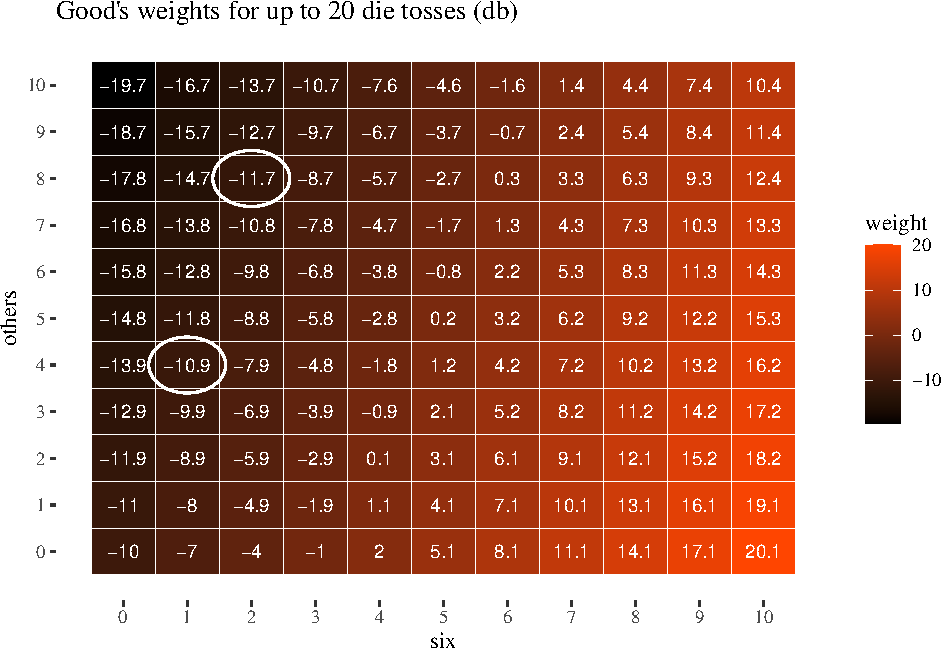
\includegraphics[width=1\linewidth]{imprecision_weight_files/figure-latex/goodWEights-1} \end{center}
\caption{Good's weights in dbs, rounded, for all possible outcomes of up to 20 tosses of a die randomly selected from 10 dice nine of which were fair, and one is \nicefrac{1}{3} loaded towards six. $H=$`the die is loaded'.}
\label{fig:goodWeight}
\end{figure}

Two facts are notable. (1) Weight can drop with sample size: for
instance the weight for 4 others and 5 sixes is 1.2db, and it is .2db
for 5 others and 5 sixes. (2) Weight can drop while the sample size
increases even if the proportion of sixes remains the same. For
instance, if none of the observations are sixes, the weights go from -10
to -19.7 as the sample size goes from 0 to 10. Less trivially, the
observation of one six in five leads to weight of -10.9, while the
observation of two sixes in ten tosses leads to weight -11.7. That is,
(Monotonicity), (Completeness), (Weak increase) and (Strong increase)
all fail for Good's measure.

Moreover, there is a conceptual difficulty in the neighborhood. Suppose
you are trying to ascertain the bias \(\theta\) of a coin, but you do
not restrict yourself to two hypotheses as in the dice example, but
rather initially take any bias to be equally likely. For each particular
hypothesis \(\theta = x\) and any set of observations \(E\) you can use
the binomial distribution to calculate \(\pr{E \vert \theta = x}\). But
to deploy Good's definition, you also need
\(\pr{E \vert \theta \neq x}\), which is less trivial, as now you have
to integrate to calculate the expected probability of the evidence given
an infinite array of possible values of \(y\). Suppose you have no
problem calculating such items. Now imagine you observe 10 heads in 20
tosses. The question `how weighty is the evidence' makes no sense here,
as Good's weight needs a hypothesis (and its negation) to be plugged in.
For this reason, in such a situation, we can at best talk about a
continuum of Good's weights, one for each particular value of
\(\theta\).

\begin{itemize}
\item
  compare to pointwise mutual information
\item
  evaluate in light of the desiderata
\end{itemize}

\hypertarget{counting-propositions}{%
\subsection{Counting propositions}\label{counting-propositions}}

Completeness, inclusion entails weight comparison, very limited
applicability

\hypertarget{skyrms-and-resilience}{%
\subsection{Skyrms and resilience?}\label{skyrms-and-resilience}}

\begin{itemize}
\tightlist
\item
\item
  relation to law Davidson Pargetter 1986, perhaps Nance, who else?
\end{itemize}

\hypertarget{imprecision-and-weight-with-intervals}{%
\subsection{Imprecision and weight with
intervals}\label{imprecision-and-weight-with-intervals}}

Keynes' later works and Peden's paper

\hypertarget{sharpening-by-richness}{%
\subsubsection{Sharpening by richness}\label{sharpening-by-richness}}

\hypertarget{sharpening-by-specificity}{%
\subsubsection{Sharpening by
specificity}\label{sharpening-by-specificity}}

\hypertarget{sharpening-by-precision}{%
\subsubsection{Sharpening by precision}\label{sharpening-by-precision}}

\hypertarget{imprecision-a-second-order-approach}{%
\subsection{Imprecision: a second-order
approach}\label{imprecision-a-second-order-approach}}

\hypertarget{information-theoretic-weight-of-evidence}{%
\subsection{Information-theoretic weight of
evidence}\label{information-theoretic-weight-of-evidence}}

\hypertarget{completeness-tends-to-improve-weight}{%
\subsection{Completeness tends to improve
weight}\label{completeness-tends-to-improve-weight}}

\hypertarget{weight-tends-to-improve-accuracy}{%
\subsection{Weight tends to improve
accuracy}\label{weight-tends-to-improve-accuracy}}

Here is a question asked by {[}COHEN 1986 TWELVE p.~276{]}: is it worth
while knowing the weight of an argument without knowing its probability?
In our terminology, questions inspired by Cohen's are: what's the point
of weight considerations if we already have the distributions? Can
weights be put to use if we do not have the distributions?

\hypertarget{literature-to-discuss}{%
\section{Literature to discuss}\label{literature-to-discuss}}

Kasser, 2016, Two Conceptions of Weight of Evidence in Peirce's
Illustrations of the Logic of Science {[}DOWNLOADED{]}

Feduzi, 2010, On Keynes's conception of the weight of evidence
{[}READ{]}

Cohen 1986, Twelve Questions about Keynes's Concept of Weight {[}READ{]}

Pedden, William 2018, Imprecise probability and the measurement of
Keynes' weight of arguments

Levi 2011, the weight of argument {[}DOWNLOADED{]}

Skyrms 1977 resiliency, propensities {[}DOWNLOADED{]}

Skyrms causal necessity, chapter on resilience {[}DOWNLOAD{]}

Synthese 186 (2) 2012, volume on Keynesian weight {[}CHECKED, NOT MUCH
ON WEIGHT ACTUALLY, NO NEED TO READ{]}

Good, weight of evidence, survey

Good, PROBABILITY AND THE WEIGHING OF EVIDENCE

David Hamer, Probability, anti-resilience, and the weight of expectation
{[}READ{]}

William Peden, Imprecise Probability and the Measurement of Keynes's
``Weight of Arguments''

Runde, Keynesian Uncertainty and the weight of arguments
{[}DOWNLOADED{]}

Weatherson, 2002, Keynes, uncertainty and interest rates
{[}DOWNLOADED{]}

Jeffrey M. Keisler, Value of information analysis: the state of
application

Edward C. F. Wilson, A Practical Guide to Value of Information Analysis

Joyce JM (2005) How probabilities reflect evidence.

\end{document}
